\documentclass[12pt,oneside,openright]{report}

\usepackage[utf8]{inputenc}
\usepackage[scaled]{helvet}
\usepackage{subcaption} % Add the subcaption package for subfigures
\usepackage{dirtytalk} %quoting package
\renewcommand\familydefault{\sfdefault} 
\usepackage[T1]{fontenc}
\usepackage{fancyhdr,xcolor}

\usepackage{graphicx} % Add the graphicx package for including images
\usepackage{geometry}
\usepackage{amsmath} % Add this line to your LaTeX preamble to use \text
\usepackage{afterpage}
\usepackage{caption}
\usepackage{float}
\usepackage{xcolor}
\usepackage[style=authoryear,backend=biber]{biblatex}
\addbibresource{bibliog.bib}
\usepackage[colorlinks=true,linkcolor=black,anchorcolor=black,citecolor=black,filecolor=black,menucolor=black,runcolor=black,urlcolor=black]{hyperref}\usepackage{graphicx}
\geometry{
  a4paper,
  left=20mm,
  right=20mm,
  top=3cm,
  headheight=4cm,
  bottom=3.5cm,
  footskip=3cm
}

\renewcommand*{\bibfont}{\footnotesize}

\newcommand{\changefont}{
    \fontsize{18}{16}\selectfont
}
\definecolor{boxcl}{HTML}{1188BB}
\definecolor{tubred}{HTML}{1188BB}



\begin{document}

\begin{titlepage}
    \centering
    % Include the image with a width of one-third of the page
    
\includegraphics[width=0.5\textwidth]{Hu-logo.png}
    \vspace{2cm}
    
    {\huge \textbf{Multisensory Integration in Virtual Reality: Effects of Passive Haptic Stimulation}\par}
    \vspace{2cm}
    {\LARGE Master Thesis\par}
    \vspace{0.5cm}
    {\textbf{submitted in fulfillment of the requirements for the degree}\par}
    Master of Science (M.Sc.)\par
    {\textbf{in the master's program ``Mind and Brain''}\par}
    \vspace{1.5cm}
    {\textbf{Humboldt-Universität zu Berlin}\par}
    {\textbf{Berlin School of Mind and Brain}\par}
    \vfill
    \raggedright
    \begin{tabular}{ll}
        \textbf{Handed in by}: & Benjamin Dupré \\
        \textbf{Date of birth:} & 26.04.1986\\
       \textbf{ Address:} & Hoppestraße 16, 13409, Berlin \\
    \end{tabular}
    \vfill
    \begin{tabular}{ll}
        \textbf{1. Supervisor:}& Dr. Michael Gaebler \\
        \textbf{2. Supervisor:}& Professor Dr. Arno Villringer  \\
    \end{tabular}
    \vfill
    {Berlin, \today \par}
\end{titlepage}

\section*{1. Introduction}
\subsection*{1.1 Problem \& Significance}
There are multiple internal signals that our nervous system processes constantly. Some of them we need to be aware of (e.g., the position of our foot), and some of them we do not need to be aware of (e.g., if our heart is contracting or expanding). Specifically, the ones we are not aware of are hard to research and understand, as they consistently operate in the background. These are the interoceptive signals—the internal stimuli generated within the organism.

From all the signals our internal ogans generate our focus will be the heart rate signal. As of late, this signal has been central to ongoing research in interoception, by looking into the effect heart-cycles have on how we process external stimuli. This influence has been extensively observed in both psychophysical and cognitive processes. For the purpose of this thesis, I will  categorize this body of literature into these two groups: the psychophysical effects and the cognitive effect of the heart cycle.

The first group, refers to the psychophysical research that looks into how heart-cycle affects perception. Mainly puting focus on relationship between physical phenomena and the perceptual effects it generates. Here, experiments with single perceptual modality and high precission measurments, have found that heart-cycle plays a crucial role in diminishing our perception of external signals in touch, vision, and auditory cues \parencite{Sandman1977-li, esra_p, AL2021118247, Grund643, motyka, Park2014}. This mutting effect has been well-documented during systolic phase and individual sensory modalities. 

Expanding on this, a recent study look into simultaneus multiple sensorial modalities \parencite{SALTAFOSSI2023108642}. The study found similar effects for multisensory integration. It showed again, that a particular heart-phase cycle impacts the timing of integration between two distinct external stimuli. In specific, the research found that paired stimuli presented during diastole heightened the level of integration for audio-tactile and visuo-tactile stimuli compared to those presented during systolic-phase. However, this effect was less pronounced for audio-visual stimuli. For these findings the authors used the Race Model Inequality (RMI) and response times (RT).Which will also be relevant variables for this study.  

The second group of studies looks into higher cognitive functions. For example, they look to measure if there is a change in how we memoryze a word when presented locked to a specific cardiac-phase —stimuli that is presented during a particular cardiac cycle is refered to phase-lock stimuli. An illustrative study is the cardiac-cycle phase-locked word retention study conducted by \Cite{Garfinkel2013-st}. On this study, it was found that words detected during systole were less effectively remembered compared to those detected during diastole \parencite{Garfinkel2013-st}. Recent variations in experimental setups, involved presenting stimuli outside phase-locked periods  \parencite{GalvezPol2018ActiveSI} in order to measure wether or not heart-cycle plays a role in our active interaction with the world. The authors found similarly, that this phenomena works also for eye seccade. It found that more eye movement occurs during systolic phases while more fixation happens during diastolic phases, thus proving also an active perceptual role. 

As we increasingly recognize the significance of cardiac-cycle phases in shaping our perception of external stimuli and cognitive functions, the connection between these two groups of research remains somewhat elusive. Efforts are directed toward constructing theories that integrate several of these observations. For instance, \parencite{AL2021118247} discusses an interoceptive predictive framework. This framework suggests that repetitive bodily signals, like the heartbeat cycle, can be predicted and suppressed to prevent entry into conscious perception, inadvertently leading to the suppression of external stimuli. Notheless it has not be tested. 

Another paper exclusivly focused on proposing a computational interoceptive predictive framework goes even further. Using a mathemathical generative model, simulated agents and synhtetic signals seeks to explain results observed in heart-rate variability literature \parencite{Allen2022}. It premises are built so that precise visual information is only available during certain parts of the cardiac cycle, which itself depends upon the state of arousal. The paper among other results, demonstrats that the model can reproduce a variety of psychological and physiological phenomena interoceptive inference literature. It offers a way to test such model. 
 
These models in the existing set-ups are hard to test. There's a need to bridge the gap not only between cognitive and psychophysical studies of interoception but also between different experimental setups. In other words, we're facing an experimental deadlock that requires enhanced ecological validity. To achieve this, a broader experimental paradigm should encompass both psychophysical stimuli and wider cognitive functions beyond perception only. In the context of this thesis, it becomes essential to simultaneously test perceptual stimulation, multisensory integration, and cognitive outcomes. Such an approach aligns experiments more closely with real-world scenarios, enhancing ecological validity and aiding our understanding of how body-brain phenomena translate into human psychology \parencite{schmuckler2001ecological}.

A tool that could facilitate ecological validity is Immersive Virtual Reality (IVR). IVR is a tool known for its effectiveness in studying cognitive processes within controlled yet complex scenarios, traditionally relies on visual displays and head-hand movement tracking. However, the integration of VR head-mounted displays with Electrocardiogram (ECG) and haptic devices presents new challenges, both practical and technical, as well as in terms of alignment with existing literature \parencite{Klotzsche2023}.

As I will detail in the following section, I expect to replicate the Redundancy Signal Effect (RSE) and Race Model Inequality (RMI) observations using IVR. This endeavor aims to validate an experimental VR setup under these conditions and extend two lines of research: multisensory integration and the influence of cardiac cycles cognition. Ultimately, this research aims to leverage Virtual Reality to bridge the gap between psychophysics findings and everyday experiences.

\subsection*{1.2 Research Topic \& Goal}

This study primary objective is to test the feasibility of incorporating touch-cardiac-cycle modulation studies into Interactive Virtual Reality (IVR) setups. IVR, being a system that often involves visual, tactile, and proprioceptive senses, inherently engages multiple senses or is intentionally designed as a multisensory experience. To facilitate a comparative analysis of results, a relevant recent study by Martina Saltafossi on vision, touch, and hearing as multisensory pairs \parencite{SALTAFOSSI2023108642} serves as a suitable reference. While there is limited research on two multisensory modalities and none to my knowledge using IVR, this study aims to bridge that gap. 

The are certain differences between the stimuli used in this study and the reference study. In this study,the only single modality is vision wereas in the reference study there are three. In this study also, the conditions are built around the sense of Touch. And Touch can be understood in many ways, therefore I will use the extended classification of tactile sensation since it provides a useful framework for understanding touch. It can be categorized into five different modes based on the presence or absence of voluntary movement: (1) tactile (cutaneous) perception, (2) passive kinesthetic perception, (3) passive haptic perception, (4) active kinesthetic perception, and (5) active haptic perception \parencite{Healy2003HandbookOP}. For this thesis, touch is defined as passive haptic perception generated by a vibrating Data-Glove.

Based on this definition, two main goals are derived:
\begin{itemize}
  \item[(i)] Assess the impact of passive haptic stimuli on reported immersion. This investigation quantifies the influence of passive haptic stimuli on questionnaire scores, shedding light on touch's role in creating a sense of presence. 
  \footnote{Saltafossi's study refers to this as "body illusions induced by multisensory conflicts between exteroceptive sensory modalities, such as vision and touch."}
    
  \item[(ii)] Confirm findings supporting the redundancy signal effect (RSE) and some aspects of the race model inequality (RMI). Checking for example the order of the cumulative distibution functions (CDF) for different RT. Additionally comparing single modal condition visual ($F_V$) and bimodal conditions were touch matches ($F_{V=T}$) or doesn’t match ($F_{V \neq T}$) the visual space. 
\end{itemize}

By examining how passive haptic stimuli influence the response time in the motor-memory task, this study seeks to replicate the overall findings of the reference paper \parencite*{SALTAFOSSI2023108642} and validate behaviorally the effects of passive haptic stimuli in a IVR motor-memory task. In a wider frame, this research aims to enhance our understanding of IVR as a research tool and further validate findings on multisensory integration and perception.

\section*{2. Methods}
    \subsection*{2.1 Participants}
    From an original pool of 23 participants that presneted to do the task we finish we 20 participats. Two of them did not fill all questionnaires and a third one was above the age limit  so we had to exclude them from the analysis, leaving us with 20 participants. The call for participants was answered considerably more by women (15) than men (5). The age across the sample was consistently around 25 years old, with the exception of one participant ($\mu=25.1 , \sigma=6.3$).
    \begin{figure}[h]
        \centering
        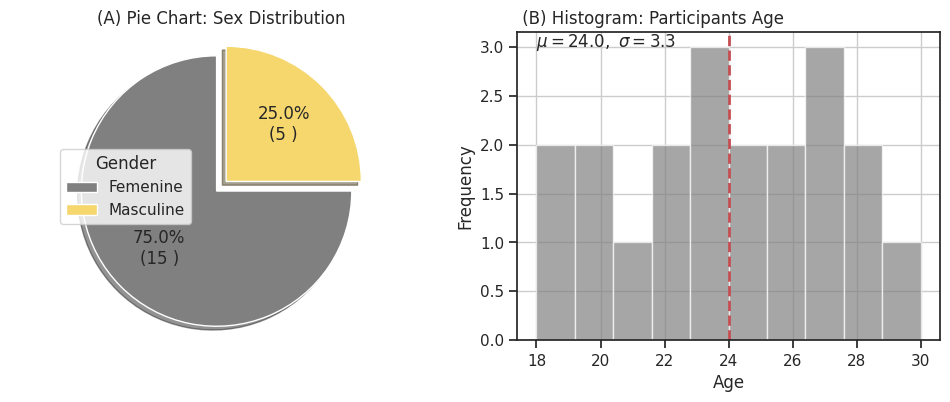
\includegraphics[width=12cm]{/home/perdices/Dokumente/Github/m-b_thesis/Analysis/figures/participants.png}
        \captionsetup{justification=justified, margin={2cm,2cm}, font={small}}
        \caption{Participants Composition}
        \label{fig:mesh1}
    \end{figure}
    
    \subsection*{2.2 Materials}
    \subsubsection*{2.2.1 Electrocardiogram (ECG):}
Heart rate data is collected using an Arduino Uno and a SparkFun Single Lead Heart Rate Monitor - AD8232. The collected data is transferred through a USB 2.0 connection and integrated into the Unity log file at a frequency of 133 Hz. Based on live ECG device \parencite{TimsECG}.

\subsubsection*{2.2.2 Head Mounted Display \& Lighthouses:}
The VR setup includes an HTC Vive head-mounted display (HMD) with two lighthouses. The headset specifications include a Dual AMOLED 3.6" diagonal display, with 1080 x 1200 pixels per eye (2160 x 1200 pixels combined), a 90 Hz refresh rate, and a 110-degree field of view. The lighthouses are equipped with SteamVR Tracking, G-sensors, gyroscopes, and proximity sensors. Both the HMD and lighthouses are connected using USB 2.0. For this study, the VR controllers were not used, and instead, hand tracking was performed using the Leap Motion sensor.

\subsubsection*{2.2.3 Leap Motion Controller:}
The Leap Motion Controller has a field of view of 150x120 degrees, with a variable range of roughly 80 cm (arm's length). It weighs 32 grams and is mounted on the HMD. The device features two 640x240 infrared cameras with a frame rate of 120 fps.

\subsubsection*{2.2.4 Data Gloves:}
The data gloves used in the study are equipped with magnetic sensors and connected to Unity using a microUSB connection. These gloves provide haptic feedback through 10 vibrotactile actuators, offering a wide range of tactile sensations with 1,024 levels of intensity. The gloves also incorporate complete finger tracking using six 9-axis Inertial Measurement Units (IMUs). These IMUs enable precise tracking of finger movements, allowing for accurate gesture recognition and enhanced interaction in virtual environments.

\subsection*{2.3 Task}

After receiving information about the COVID rules and the experiment, participants engaged in the following tasks:

\begin{enumerate}
\item[(i)] \textbf{Questionnaires:} Before the IVR experience, participants completed the Edinburgh Handedness Questionnaire and the PRE-Cybersickness Questionnaire. Following the IVR experience, participants filled out the Virtual Reality Subjective Evaluation Questionnaire and POST-Cybersickness Questionnaire.

\item[(ii)] \textbf{Heartbeat Count Task (HCT):} Participants performed a one-minute heartbeat count task before and after the IVR task. Note that this task is not considered within this thesis.
\end{enumerate}

Following the completion of the initial questionnaires and HCT, participants moved to another room where the IVR (Immersive Virtual Reality) equipment was set up. This included a head-mounted display (HMD), data gloves, and an ECG (Electrocardiogram) device. Participants received a brief training session before proceeding with the heartbeat count task and the IVR memory-motor task.

The IVR Memory-Motor Task comprised the following steps:
\begin{enumerate}
    \item[\textbf{a.}] Participants stood in front of a virtual table, allowing ample time to acclimate to the virtual environment, as depicted in Figure \ref{fig:look}.
    
    css
    
    \item[\textbf{b.}] Prior to each trial, a new calibration process started. Participants placed their palms facing up within the shadowed hands, ensuring the standard positioning. Refer to Figure \ref{fig:look} (b) for the calibration setup.
    
    \item[\textbf{c.}] Participants viewed a two-dimensional sketch (Figure \ref{fig:look} (c)) displayed in the virtual environment, prompting them to memorize the red ball's position. During this phase, participants kept their virtual hands open with palms facing up.
    
    \item[\textbf{d.}] The sketch disappeared, and a red ball appeared from the top, landing in either of the participant's hands. Participants then observed a template on the table, resembling the initial sketch they memorized. Their task was to place the ball in the correct location on the template as swiftly as possible.
    
    \end{enumerate}

    \begin{figure}[!ht]
        \centering
        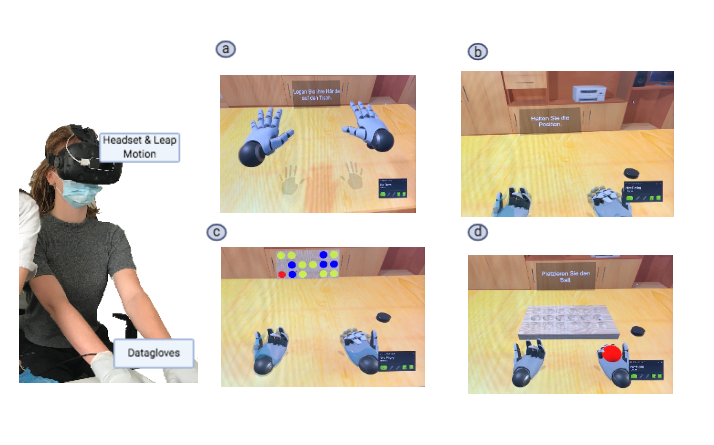
\includegraphics[width=15cm]{/home/perdices/Dokumente/Github/m-b_thesis/Analysis/figures/design_ilustration.png}
        \captionsetup{justification=justified, margin={2cm,2cm}, font={small}}
        \caption{Illustration of the IVR Memory-Motor Task: (a) represents the acclimation period during initial setup; (b) showcases the first-person perspective of the calibration phase; (c) displays the 2D sketch for memorizing ball position; (d) presents the appearance of the ball and the 3D template for ball placement, marking the beginning of each trial.}
        \label{fig:look}
        \end{figure}
 
In 108 trials, three conditions—congruent ($V=T$), incongruent ($V \neq T$), and visual-only ($V$)—were randomly presented 36 times each, appearing rapidly in succession. The initiation of each trial was marked by placing the ball in a hand, and its conclusion was noted when the ball reached its designated location on the template (see Figure \ref{fig:look}).Additionally, as mentioned before after thte IVR test final round of questionnaires intended for repeated measures on sickness and initial assessment of the immersion experienced with the haptic glove and hands.

\subsection*{2.4 Mesurements}
\subsubsection*{2.4.1 Immersive Virtual Reality (VR):}

The VR experience was presented and tracked using an HTC Vive head-mounted display (HMD), two lighthouses, a Leap Motion sensor, and Haptic Data Gloves. Movement data from the data gloves, Leap Motion device, and the HMD was collected. For movement analysis, only the wrist movements tracked by the Leap Motion device were considered, excluding the fingertips' magnetic tracking sensor data. All movements were recorded in a Euclidean coordinate system (X, Y, Z) with the original calibrating point set at (0, 0, 0). This provided a total of nine streaming sources of data (e.g., Headset X, Headset Y, Headset Z, and so on). Notably, rotational data was not included in the analysis.

Additionally, in the game output data, there are flags that signal if a button was pressed, if the ball is placed in the holder, and when the trial started.

\subsubsection*{2.4.4 Electrocardiogram (ECG):}

Heart rate data was collected using a USB cable and integrated into Unity Engine. This information was coupled with all other Unity data at a frequency of 133 Hz.

\subsubsection*{2.4.3 Questionnaires:}

\begin{enumerate}
\item[(i)] Virtual Reality Subjective Evaluation Questionnaire: This self-made questionnaire consists of 26 items oriented towards capturing whether the VR experience felt real for the participant or not. It explores the level of engagement, hand movement, task difficulty, and other controlling factors. The questionnaire uses a Likert scale ranging from one to seven.
\item[(ii)] PRE/POST-Cybersickness Questionnaire: The version applied in this study is a shorter adaptation of the simulator sickness questionnaire (SSQ) \parencite*{avpsy}. It employs a Likert scale ranging from one to four, with labels going from "not present," "somewhat," "clearly," and "very strongly." The questionnaire includes 16 items based on symptoms, such as "fatigue" and "general discomfort," among others.
\end{enumerate}

\subsection*{2.5 Data Analysis}

All response times were measured from the moment the ball entered the scene in the trial until the moment it "exploded". Trials where the error button was pressed were excluded from the analysis. Prior to analysis, outlier correction was performed by removing data points that deviated more than 3 × 1.4826 times the median absolute deviation (MAD) from the median, equivalent to 3 standard deviations assuming a normal distribution \parencite{Innes2019ACA}. No responses were removed due to being too fast. However, 13\% of trials were eliminated due to excessive slowness. The final sample consisted of 1826 response times (approximately 24 per condition per participant). After the removal of outliers, the response times for each condition were converted into rates (1/RT). Prioritizing normality in the error distribution over other factors, such as the scale of properties or interacting effects, was considered crucial for this proof of concept, emphasizing the essential validity of the experimental conditions. 

To enable comparisons with Saltafossi's reference paper, our aim was to confirm the well-established redundant signal effect — indicating faster response times to bimodal stimulation compared to single stimulation — and partially construct the Race model Inequality to validate its applicability across all time periods $t$.

To achieve this, I followed the methodologies outlined in \cite{Ulrich2007,Innes2019ACA}. Given one individual stimulus and two bimodal stimuli, a simplified version without the "bounding sum" . The process involved three steps. First, empirical cumulative density functions (CDFs) were constructed for all three conditions (Bimodal pairs: ($F_{V=T}$), ($F_{V \neq T}$), and Single Signal: ($F_V$)). Second, percentiles were determined. Third, aggregation across participants involved computing separate paired t-tests at each percentile under examination. For a detailed breakdown of the calculations, please refer to \cite{Ulrich2007}.

\section*{3. Results}
\subsection*{3.1 Assessing the Impact of the Haptic Glove on Reported Immersion}
    
    Nineteen respondents answered 27 questions, rating them on a scale from 1 (Does Not Apply) to 7 (Totally Applies). The key findings from the questionnaire are as follows:
    
    \begin{enumerate}
        \item In question number 24, the perceived increase in immersion due to the haptic gloves was high ($\text{Mdn} = 6$, $\mu = 6$, $\sigma = 0.76$). Furthermore, the task was considered enjoyable at least some of the time ($\text{Mdn} = 6$, $\mu = 5.4$, $\sigma = 1.04$).
        
        \item Question 26 revealed that haptic feedback was perceived as either not significantly improving performance or having a neutral effect ($\text{Mdn} = 3$, $\mu = 3.6$, $\sigma = 1.49$). Similarly, in question 12, the perception of haptic feedback improving response time was generally rated as neutral to not applicalbe ($\text{Mdn} = 3$, $\mu = 3.7$, $\sigma = 1.74$). In question 7, when asked about the impact on results, haptic feedback was perceived as not applicable ($\text{Mdn} = 6$, $\mu = 6$, $\sigma = 0.76$).
    
        \item Notably, the assertion that it was very challenging to remember the position of the red ball ($\text{Mdn} = 2$, $\mu = 2.9$, $\sigma = 1.45$) was generally disagreed upon. Conversely, in question 8, which asked about the ease of remembering the location of the red ball, responses were as expected ($\text{Mdn} = 5$, $\mu = 5.1$, $\sigma = 1.37$).
    
        \item The highest variance was observed in question 13 ($\text{Mdn} = 5$, $\mu = 4.2$, $\sigma = 1.79$), indicating that haptic feedback made it easier to place the ball. Similarly, question 18, which inquired about the ease of counting heartbeats at the beginning of the experiment, also showed significant variance ($\text{Mdn} = 4$, $\mu = 4$, $\sigma = 1.79$). 
        
    \end{enumerate}
    
    For more details please go to the supplement section 

    
\subsection*{3.2 Touch stimuli influence the response time}
\subsubsection*{3.2.1 General Performance}

First, I examined the mistake rates in ball placement per condition to ensure they did not significantly affect the experiment. In the visual-only condition ($V$), the mistake rate was $6.35\%$ ($\pm 0.99\%$, SEM), for the visual incongruent touch condition ($V \neq T$), the mistake rate was $5.79\%$ ($\pm 0.59\%$), and for the visual congruent touch condition ($V=T$), it was $6.91\%$ ($ \pm 1.93\%$). However, a one-way ANOVA (feedback type) revealed no significant effects ($ F \leq 0.08$, $p \geq 0.91$). Although the task is notably more complex than mere stimulus recognition, these mistake rates remain notably low and were not subjected to further analysis.

To assess whether the experimental manipulations mimicked the diversity of Redundancy Signal Effect (RSE)  studies, we next tested A one-way repeated-measures ANOVA. Using the previously mentioned transformations, the test demonstrated a significant main effect for stimulus ($F(2,38) = 3.4$, $p \leq 0.043$, $\eta p^2 = 0.15$). The median response time for the `Congruent` condition ($V=T$) was the fastest ($3236$ ms $\pm 456$ ms), followed by the `Incongruent` ($V \neq T$) condition ($3268$ ms $\pm 470$). The slowest condition was observed in the absence of haptic stimuli `None` ($V$) ($3284$ ms $\pm 463$). Hence, the experimental conditions effectively influenced response times as shown in figure \ref{fig:error}.

\begin{figure}[!ht]
    \centering
    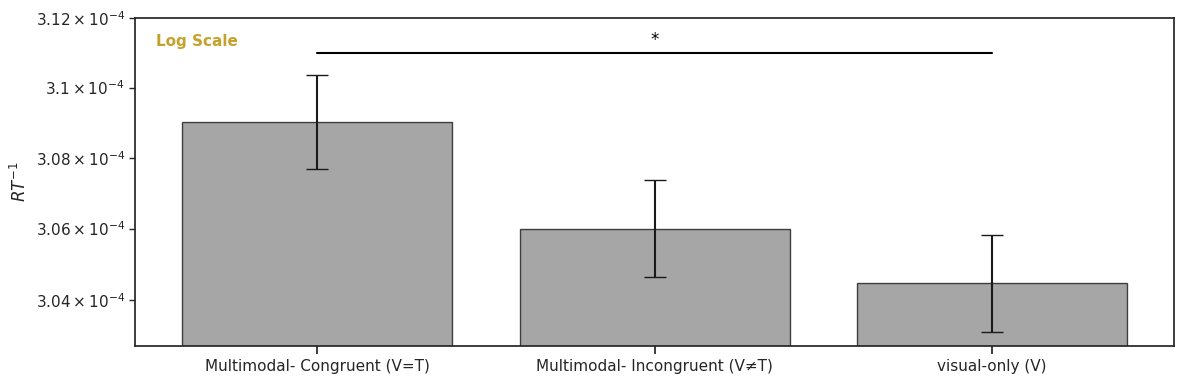
\includegraphics[width=12cm]{/home/perdices/Dokumente/Github/m-b_thesis/Analysis/figures/bar_erros_bars_stimulus_constructions.png}
    \captionsetup{justification=justified, margin={2cm,2cm}, font={small}}
    \caption{One-way repeated-measures ANOVA using $RT^{-1}$. The test revealed a significant main effect for the conditions ($F(2,38) = 3.4$, $p \leq 0.043$, $\eta p^2 = 0.15$)}
    \label{fig:error}
\end{figure}

However, post hoc Tukey HSD tests did not show any specific pairwise differences. While there is an overall difference between conditions, the specific pairwise differences were not identified

Given the absence of identified specific pairwise differences in the post hoc analysis, I decided to conduct a more comprehensive investigation using a Generalized Linear Mixed Model (GLMM). Although this method was not used in the referenced paper, it offers numerous advantages in multilevel research designs. Particularly, as it addresses the following issue:

\textit{"A linear relationship between the standard deviation of RTs and mean RT demonstrated in many previous studies of RT in binary choice tasks. This linear relationship is also evident in plots of the residuals, indicating heteroscedasticity in LMM analyses, characterized by an increasing spread in residuals for longer predicted RT"} \parencite{Lo2015-fv}.

By using GLMM, rather than imposing normality and eliminating error deviation, we allow to use a distributions that matchs the properties of the mesuared RT \parencite{Lo2015-fv}. To do this, I utilized the \textit{statsmodels} statistical package in Python, the \textit{mixedlm} function. Other similar studies use the same method \parencite{RSE_FBI}.

The following were the chareceristics of the mixed linear model analysis conducted. It aimed to assess the impact of feedback types (($V=T$), ($V \neq T$), ($V$)) on response times. The model included feedback type as a fixed effect and participant as a random effect, 'congruent' feedback type served as the reference category.

The model coefficient for the 'none' ($V$) feedback type ($\beta = 45.726, SE = 22.594, p = 0.043$) reached statistical significance at the conventional level ($\alpha =0.05 $) when compared to the 'congruent' ($V=T$) feedback type. This suggests a significant difference in response times between the 'none' and 'congruent' feedback types. The coefficient for 'incongruent' feedback type ($\beta = 32.975, SE = 22.686, p = 0.146$) did not reach conventional levels of significance. 

Thus, the congruent condition demonstrated significantly faster performance compared to the visual-only condition. This outcome aligns with the expected results according to the RSE. However, the findings present a mixed perspective. Despite this significant contrast, the more stringent post hoc Tukey HSD tests revealed no notable differences between pairwise conditions. Additionally, the GLMM indicated significance solely between the congruent and visual-only ($V=T$ - $V$) conditions and not between then congruent and incongruent conditions ($V=T$ - $V \neq T$). To understand if this mixed results are due to the irrelevancy of the condition 'incongruent' ()$V \neq T$) or the result of change behavior ovet time, we can llok into the CDF grapf. 

\subsubsection*{3.2.2 Redundancy Signal Effect and Multisensory Integration}

As mention in the methods section, the experiment does not allow for a full test of the RMI, but for a partial test of the RSE. This becuase there is not single modality for tactile sense in the experiental set-up. We already saw that the General Performance showed a partial respect the RSE. Only between the congruent and the visual-only conditions. No significant results were found between the incongruent and the visual only condition. 

\begin{figure}[!ht]
    \centering
    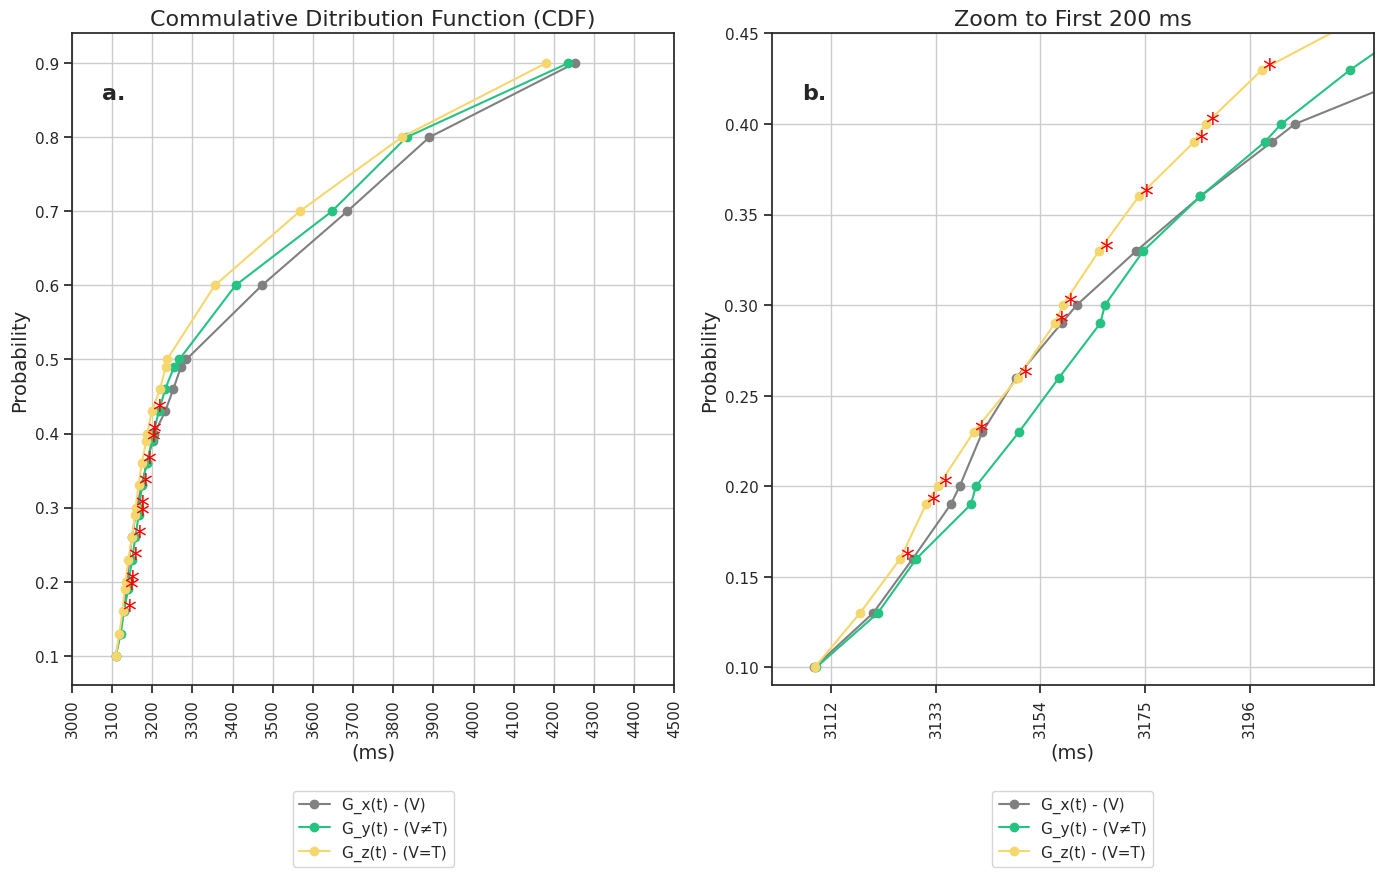
\includegraphics[width=12cm]{/home/perdices/Dokumente/Github/m-b_thesis/Analysis/figures/CDF.png}
    \captionsetup{justification=justified, margin={2cm,2cm}, font={small}}
    \caption{ (a.) Displays the 10 estimated percentile points for each of the three functions of interest: Gx, Gy, Gz, considering all participants. (b.) Is a zoom in the first 200 ms. Acording to the RSE, the visual $V$ type should be under Gy, Gz at all moments. Our data shows that is not the case for the RT in the first 200 ms.}
    \label{fig:CDF}
\end{figure}

In figure \ref{fig:CDF} we can see the RT distributions for all three conditions. With a second panel looking into more detail for the first 200 ms of reponse. First given the results in the first half I will test if th differences observed between Gx (CDF for visual-only condition) and Gz (CDF for Congruent condition) obtained for every participant, are significant overall for each Percentile estimation. When runnnig a paired one-sided t-test the difference  was significant for:


\begin{table}[!ht]
        \centering
        \begin{tabular}{lcc}
        \hline
        \textbf{Percentile Estimation} & \textbf{t-value} & \textbf{p-value} \\ \hline \hline
        0.16  & 1.88  & 0.04 \\
        0.19  & 2.04  & 0.03 \\
        0.2   & 2.01  & 0.03 \\
        0.23  & 1.97  & 0.03 \\
        0.26  & 2.06  & 0.03 \\
        0.29  & 2.03  & 0.03 \\
        0.3   & 2.02  & 0.03 \\
        0.33  & 2.11  & 0.02 \\
        0.36  & 2.08  & 0.03 \\
        0.39  & 1.83  & 0.04 \\
        0.4   & 1.79  & 0.04 \\
        0.43  & 1.74  & 0.05 \\
        \hline
        \end{tabular}
        \captionsetup{justification=justified, margin={2cm,2cm}, font={small}}
        \caption{Significant differences between Gx and Gz for each percentile using the results of t-tests.}
        \label{tab:significant-results}
\end{table}
    

\pagebreak
\section*{4. Discussion}

This thesis aimed to test the feasibility of using IVR for studying heart-cycle modulation and bridging the existing gap between cognitive and psychophysical research. To achieve this goal, the thesis employed an IVR memory task wherein participants were tasked with remembering a location and immediately placing a red ball over this location in a 3D template. The study utilized a within-subject experimental design with three categories: congruent visual-tactile stimuli, incongruent visual-tactile stimuli, and visual-only stimuli. Reaction Time (RT) and Accuracy were the measured parameters.

To build the comparison, I followed the steps outlined in my reference studies \parencite{Innes2019ACA, SALTAFOSSI2023108642, Ulrich2007}. Again is important to mention that there is only one single modality stimuli ($V$), thus limits the RMI comparisons. The initial step involved testing the validity of stimulus construction by analyzing and modeling reaction times to uni-modal and bi-modal stimuli. My results indicated that responses to multisensory pairs ($V=T$), ($V \neq T$) were faster than those to unimodal stimuli ($V$). This observation in VR mirrors the redundant signal effect, suggesting that redundant conditions (two sensory signals) elicit quicker reaction times compared to the single sensory condition \parencite*{SALTAFOSSI2023108642}.

There were, however, mixed results in significance for the incongruent case ($V \neq T$). When attempting to identify pairwise differences through a Tukey HSD test, no significant differences were found. Subsequently, running a GLMM confirmed a difference between the congruent ($V=T$) and unimodal visual cases ($V$), but not for the incongruent ($V \neq T$).

\Cite{RSE_FBI} proposes a plausible explanation for the absence of a difference in the RSE between congruent and incongruent conditions. It suggests that the mere simultaneous occurrence of visual and vibrotactile stimuli might suffice to result in multisensory integration, irrespective of whether these multisensory stimuli are functionally linked at a higher level or not (e.g., touch in the hand holding the ball). An alternative explanation could be that the discrepancy observed in the incongruent case is so marginal that the statistical power of the present study might not be sufficient to detect it significantly.

Regarding the power of the study, one conclusion is that, due to considerations of ecological validity, each trial in our IVR study spans a longer time frame compared to traditional psychophysics experiments (with a mean duration of 3400 ms as opposed to the typical 200 ms). This extended duration contributes to increased variance and skewness in response times (RT). Moreover, according to the literature, the influence of the cardiac cycle on stimuli ranges from 10 to 40 ms, posing a challenge when investigating its effects in IVR environments. Consequently, the statistical power of future research needs to be increased threefold, considering, for instance, involving 60 participants, especially if an additional condition related to heart cycles is to be included in the analysis.




%-------- CREATING BIBLIOGRAPHY

%\bibliographystyle{plain} % Choose your style
%\bibliography{bibliog.bib}  % Use your actual .bib file name

\newpage
\section*{Supplement}
    \begin{figure}[H]
        \centering
        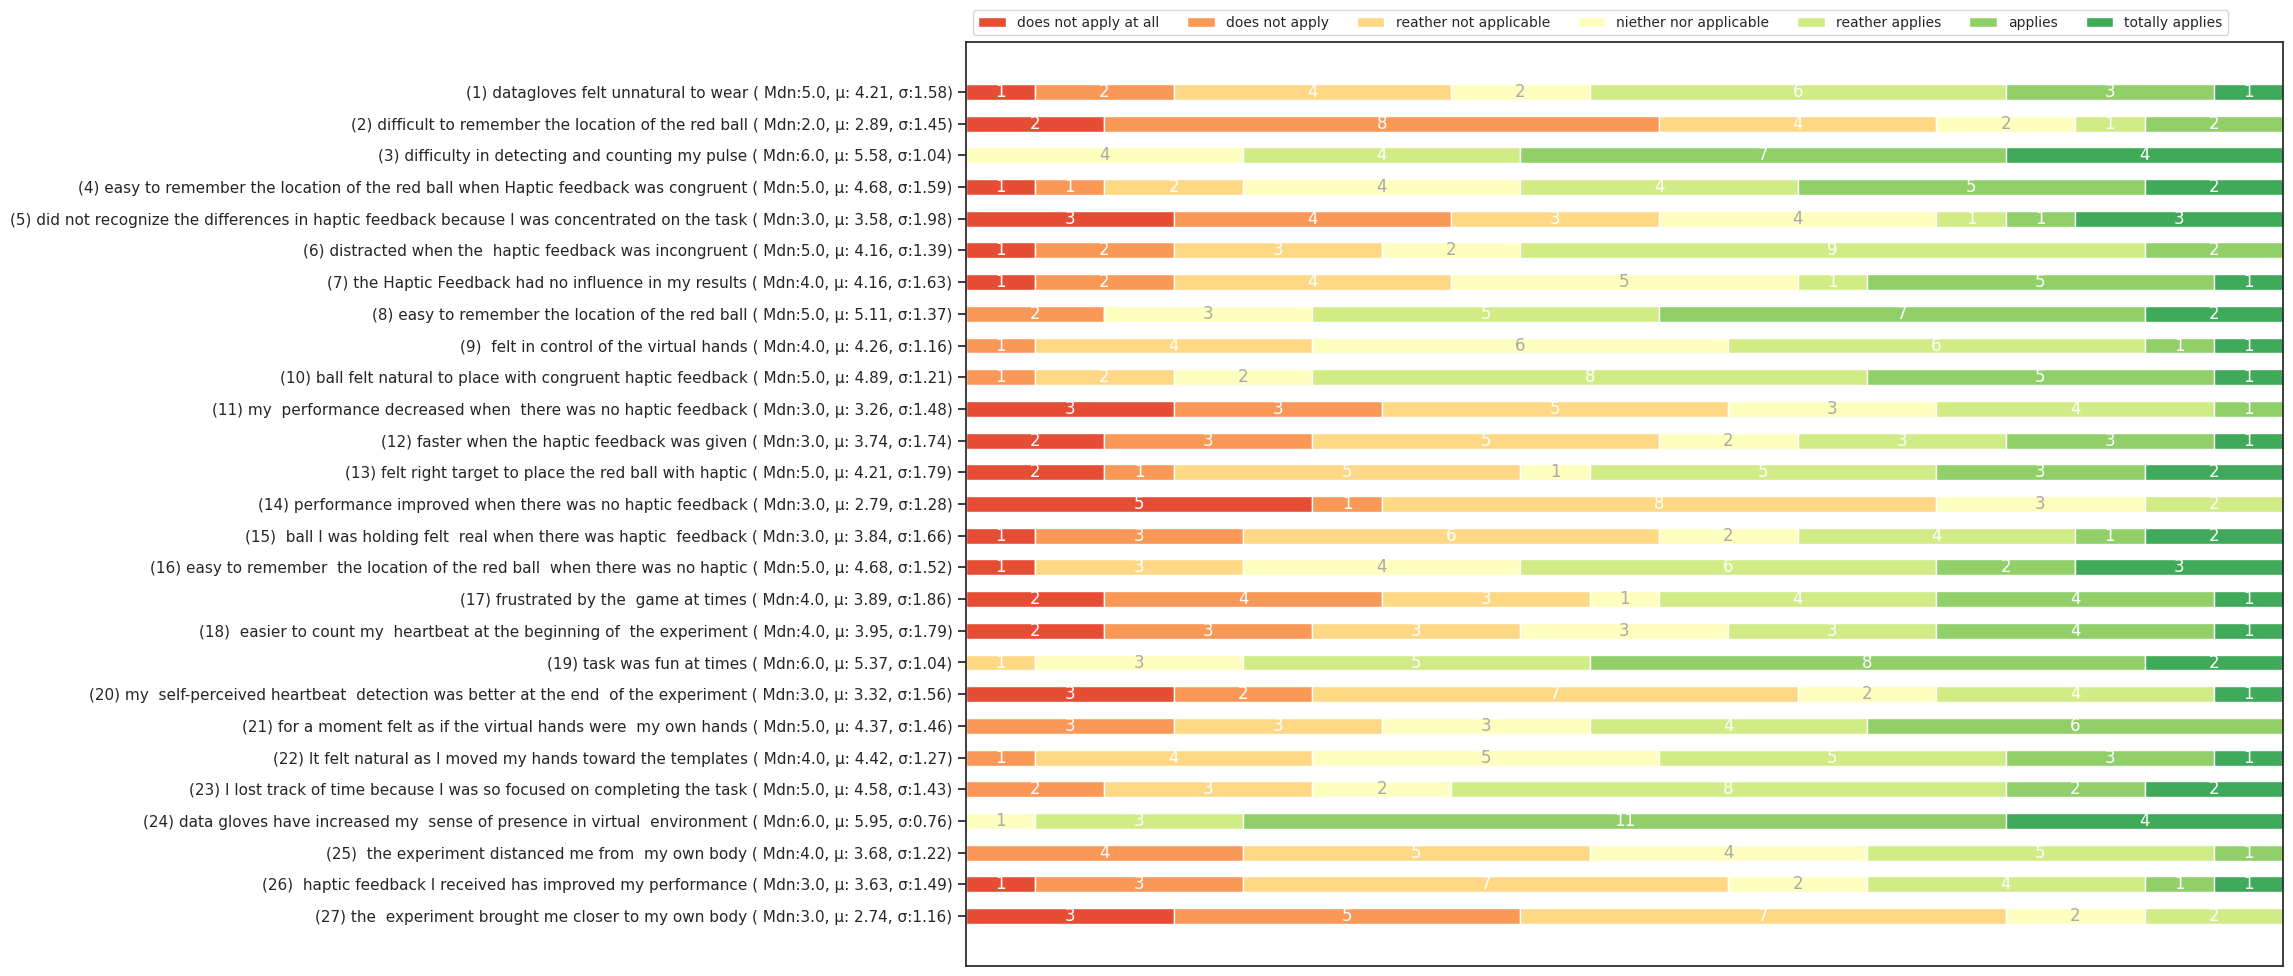
\includegraphics[angle=90, width=\textwidth, height=20cm, keepaspectratio]{/home/perdices/Dokumente/Github/m-b_thesis/Analysis/figures/questionaire_fig.png}
        \captionsetup{justification=justified, margin={2cm,2cm}, font={small}}
        \caption{Results: Virtual Reality Subjective Evaluation Questionnaire}
        \label{fig:quest}
    \end{figure}
\pagebreak


\paragraph{\textbf{References}}
\printbibliography[heading=none]

\end{document}

